\section{Key Network Parameters and Derived Cost Functions}
\label{ch1:sec:key-network-parameters}

In literature (see Chapter \ref{ch-review}), two distinct approaches have been used to improve performance of a system.
Either cost is reduced or utility is maximised.
Both approaches rely on a mathematical explanation of the underlying features that relate to performance of the system.
To reiterate, utility ought to be maximised, since the benefit of the underlying mechanisms ought to be increased to a maximum, whereas cost should be minimised.
The choice for this piece of work was to relate key network parameters to associated cost functions, with the reason that a cost can be minimised to a finite value of zero.
This means that solutions to a cost function, where the resulting cost is zero, are by definition optimal solutions, whereas a utility function can have multiple maxima that need not be the best solution.
To illustrate this feature, an arbitrary utility function, $\zeta^{*}(x)$, and cost function, $\zeta(x)$, have been plotted in Figures \ref{ch1:subfig:sketch-utility} and \ref{ch1:subfig:sketch-cost}, respectively.

\begin{figure}\centering
	\subfloat[Sample utility function]{%
		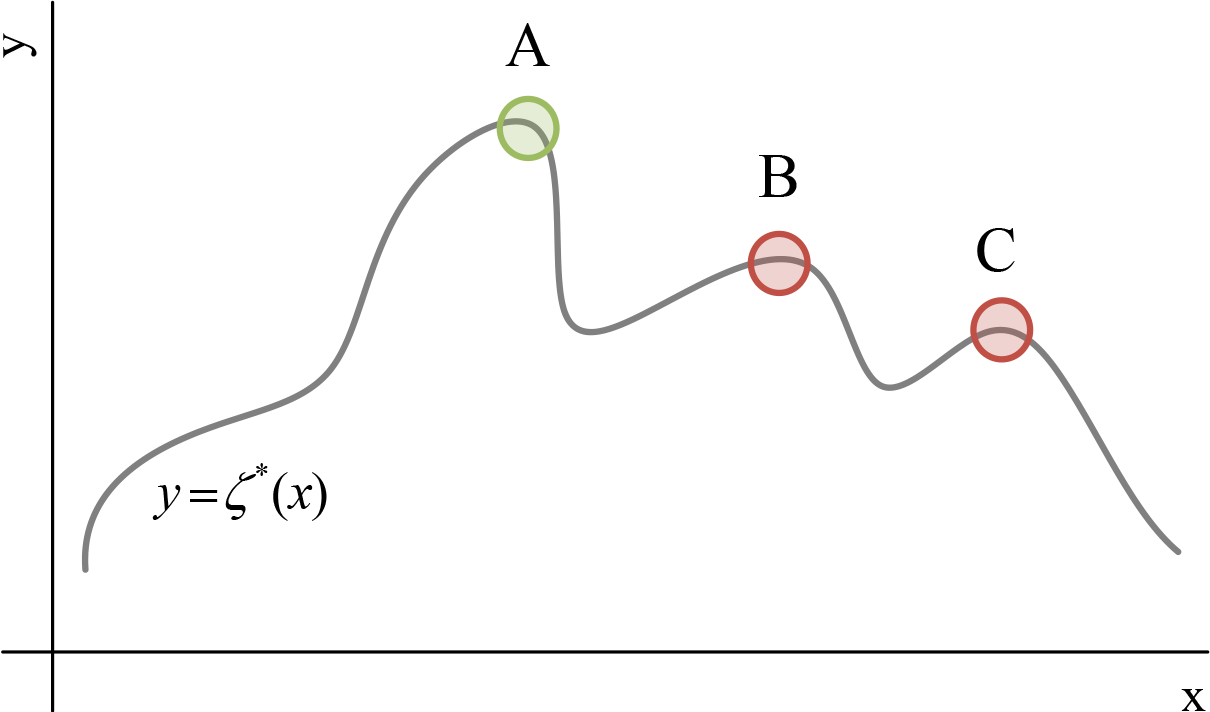
\includegraphics[width=0.45\textwidth]{_chapter1/fig/sketch-utility}%
		\label{ch1:subfig:sketch-utility}%
		}
	\hspace{5mm}
	\subfloat[Sample cost function]{%
		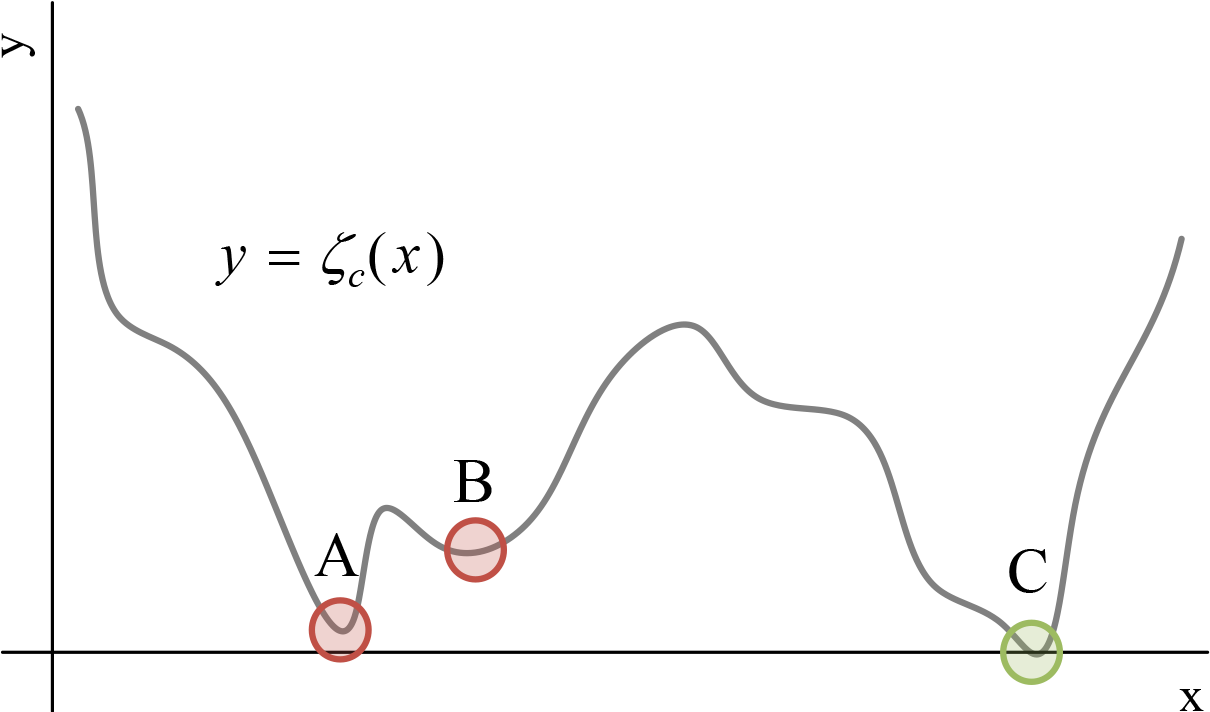
\includegraphics[width=0.45\textwidth]{_chapter1/fig/sketch-cost}%
		\label{ch1:subfig:sketch-cost}%
		}
	\caption{Benefit of using cost function over utility function}
	\label{ch1:fig:sketch-utility-vs-cost}
\end{figure}

Again, these two figures illustrate how the peaks of the utility function are at different, large values of $y$, whereas the troughs of the cost function always approach zero.
Depending on the starting condition, i.e. the initial values for $x$, different maxima or minima (i.e. points $A$, $B$ or $C$) may be found.
Here, the best solution for $\zeta^{*}(x)$ is at point $A$, whereas the best solution for $\zeta(x)$ is at point $C$.
Whilst point $A$ represents the highest utility, it does not imply optimum system performance, as utility is unbounded, i.e. $\zeta^{*}(x) \in (-\infty, \infty) \forall x$.
In contrast, for the cost function, point $C$ would represent an absolute minimum, since a cost function's range is greater or equal to zero, i.e. $\zeta(x) \geq 0 \forall x$.
Therefore, the cost's proximity to zero directly indicates the system performance (whilst the utility's proximity to infinity would not make sense).

With this in mind, the key network parameters can be explained and the corresponding cost functions can be defined.
The choice of parameters is virtually inexhaustible since one could treat every single current, voltage or phase angle as a potential network parameter.
In reality (particularly in the context of NTVV), a power distribution network could only be probed at two points: the substation and the ESMU.
Therefore, all these possible measurements and the derived parameters are treated as key network parameters; these parameters are from hereon referred to as ``realistic parameters''.
For the work presented in this chapter, all realistic parameters are extracted from power flow simulations.

In this simulation of a power distribution network (i.e. in OpenDSS), a system of nodal power flow equations is solved.
In the IEEE LV Test Case, there are 906 three phase buses, resulting in 2718 nodes for which current and voltage can be obtained.
This abundance of values means that a lot of additional parameters, that could not easily be measured in reality may also be included in the set of key network parameters; these parameters are from hereon referred to as ``theoretical parameters''.
To restrict the amount of theoretical parameters, they were chosen based on their importance and impact on actual network operation.

A list of both realistic and theoretical key network parameters\footnote{A key network parameter is marked with a dagger ($\dagger$) if it is a theoretical parameter that can only be extracted form power flow simulations.} is presented below, before going into detail for each parameter:

\begin{itemize}
	\item Voltages at substation transformer's secondary winding
	\item Voltages at ESMU's PCC
	\item Voltages at customer lateral$^{\dagger}$
	\item Total power flow
	\item Line utilisation
	\item Distribution losses$^{\dagger}$
\end{itemize}

\subsection{Voltages at substation}
\label{ch1:subsec:voltages-at-substation}

In UK LV distribution networks, the substations supply power to the feeding cable.
Substations provide the link from MV distribution network, which operates at 11kV P2P, to the LV distribution network, which operates at 230V P2N (i.e. 400V P2P).
If the substation transformer was an ideal transformer, then the voltage measured at its secondary winding would remain constant.
In reality however, the internal losses (e.g. conductive losses and magnetic leakage) lead to a drop in voltage with increasing load.
Therefore, any deviation from the substation's nominal voltage may be a result of suboptimal network operation.

If one defines the substation voltage as a single phase voltage $v_{ss,p}(t)$, where $p$ is the phase number and $t$ the time at which the measurement was taken, then a divergence cost can be calculated as $\zeta_\text{voltage}(v_{ss,p}(t)) \forall t$.
This cost is defined as:

\begin{equation}
\begin{split}
	\zeta_\text{voltage}(\textbf{v}(t)) :=& \sum_{\phi=1}^{\Phi}{\begin{cases}
		\zeta_h(v_{\phi}(t)) & \text{if } V_{ss} \leq v_\phi\\
		\zeta_l(v_{\phi}(t)) & \text{otherwise}\\
	\end{cases}} \forall t\\
	&\text{ where } \Phi \in \mathbb{Z}^{>0}
\end{split}
\label{ch1:equ:voltage-deviation}
\end{equation}

In this voltage cost function, $\Phi$ represents the number of phases (i.e. $\Phi = 3$), and $\zeta_h(v)$ and $\zeta_l(v)$ are two functions that convert a single voltage value, i.e. $v_p$, into a normalised positive cost based upon the direction of voltage deviation.
E.g. if the voltage $v_p$ is greater than or equal to the nominal substation voltage, $V_{ss}$, then the result from $\zeta_h(v)$ is used as a cost; otherwise the result from $\zeta_l(v)$ is used.
In order to define these two functions, the corresponding high and low voltage thresholds, respectively $V_h$ and $V_l$, are introduced.
With those high and low voltage bands, $V_{ss}$ has to be chosen in order to satisfy the following inequality:

\begin{equation}
	V_l < V_{ss} < V_h
\end{equation}

For the presented work, these two voltage thresholds are based on the UK's nominal LV voltage range of +10\% -6\% around $V_n$, i.e. 230V P2N.

\begin{equation}
	\zeta_h(v) := \alpha \left|\frac{v-V_{ss}}{V_h-V_{ss}}\right|^{\beta}
	\label{ch1:equ:high-voltage-threshold-cost-complete}
\end{equation}

\begin{equation}
	\zeta_l(v) := \alpha \left|\frac{V_{ss}-v}{V_{ss}-V_l}\right|^{\beta}
	\label{ch1:equ:low-voltage-threshold-cost-complete}
\end{equation}

In this context of defining $\zeta_{voltage}$, the variable $\alpha$ is used as the functions' linear weight that scales the corresponding cost, and the variable $\beta$ linearly increases the functions' gradients as voltage continues to deviate.
More specifically, $\alpha$ determines the value of the functions at voltages $V_l$ and $V_h$, where $\alpha \in \mathbb{R}^{>0}$; for example, when $\alpha = 1$, then $\zeta_{h}(v_l) = 1$.
$\beta$ on the other hand may take any value in the range of $\mathbb{R}^{>2}$, to assure a continuously differentiable cost function.
Both $\alpha$ and $\beta$ were treated as constants and, for the scope of this work, set to $1$ and $2$, respectively.
Substituting these values into Equations \ref{ch1:equ:high-voltage-threshold-cost-complete} and \ref{ch1:equ:low-voltage-threshold-cost-complete}, simplifies the high and low cost functions to:

\begin{equation}
	\zeta_h(v) := \left|\frac{v-V_{ss}}{V_h-V_{ss}}\right|^{2}
	\label{ch1:equ:high-voltage-threshold-cost-simple}
\end{equation}

\begin{equation}
	\zeta_l(v) := \left|\frac{V_{ss}-v}{V_{ss}-V_l}\right|^{2}
	\label{ch1:equ:low-voltage-threshold-cost-simple}
\end{equation}


Since voltage levels drop continuously along a purely consumptive feeder, substations may boost the voltage towards the upper threshold.
The behaviour of boosting $V_{ss}$ on the cost function $\zeta_\text{voltage}(v)$ is shown below.

\begin{figure}\centering
	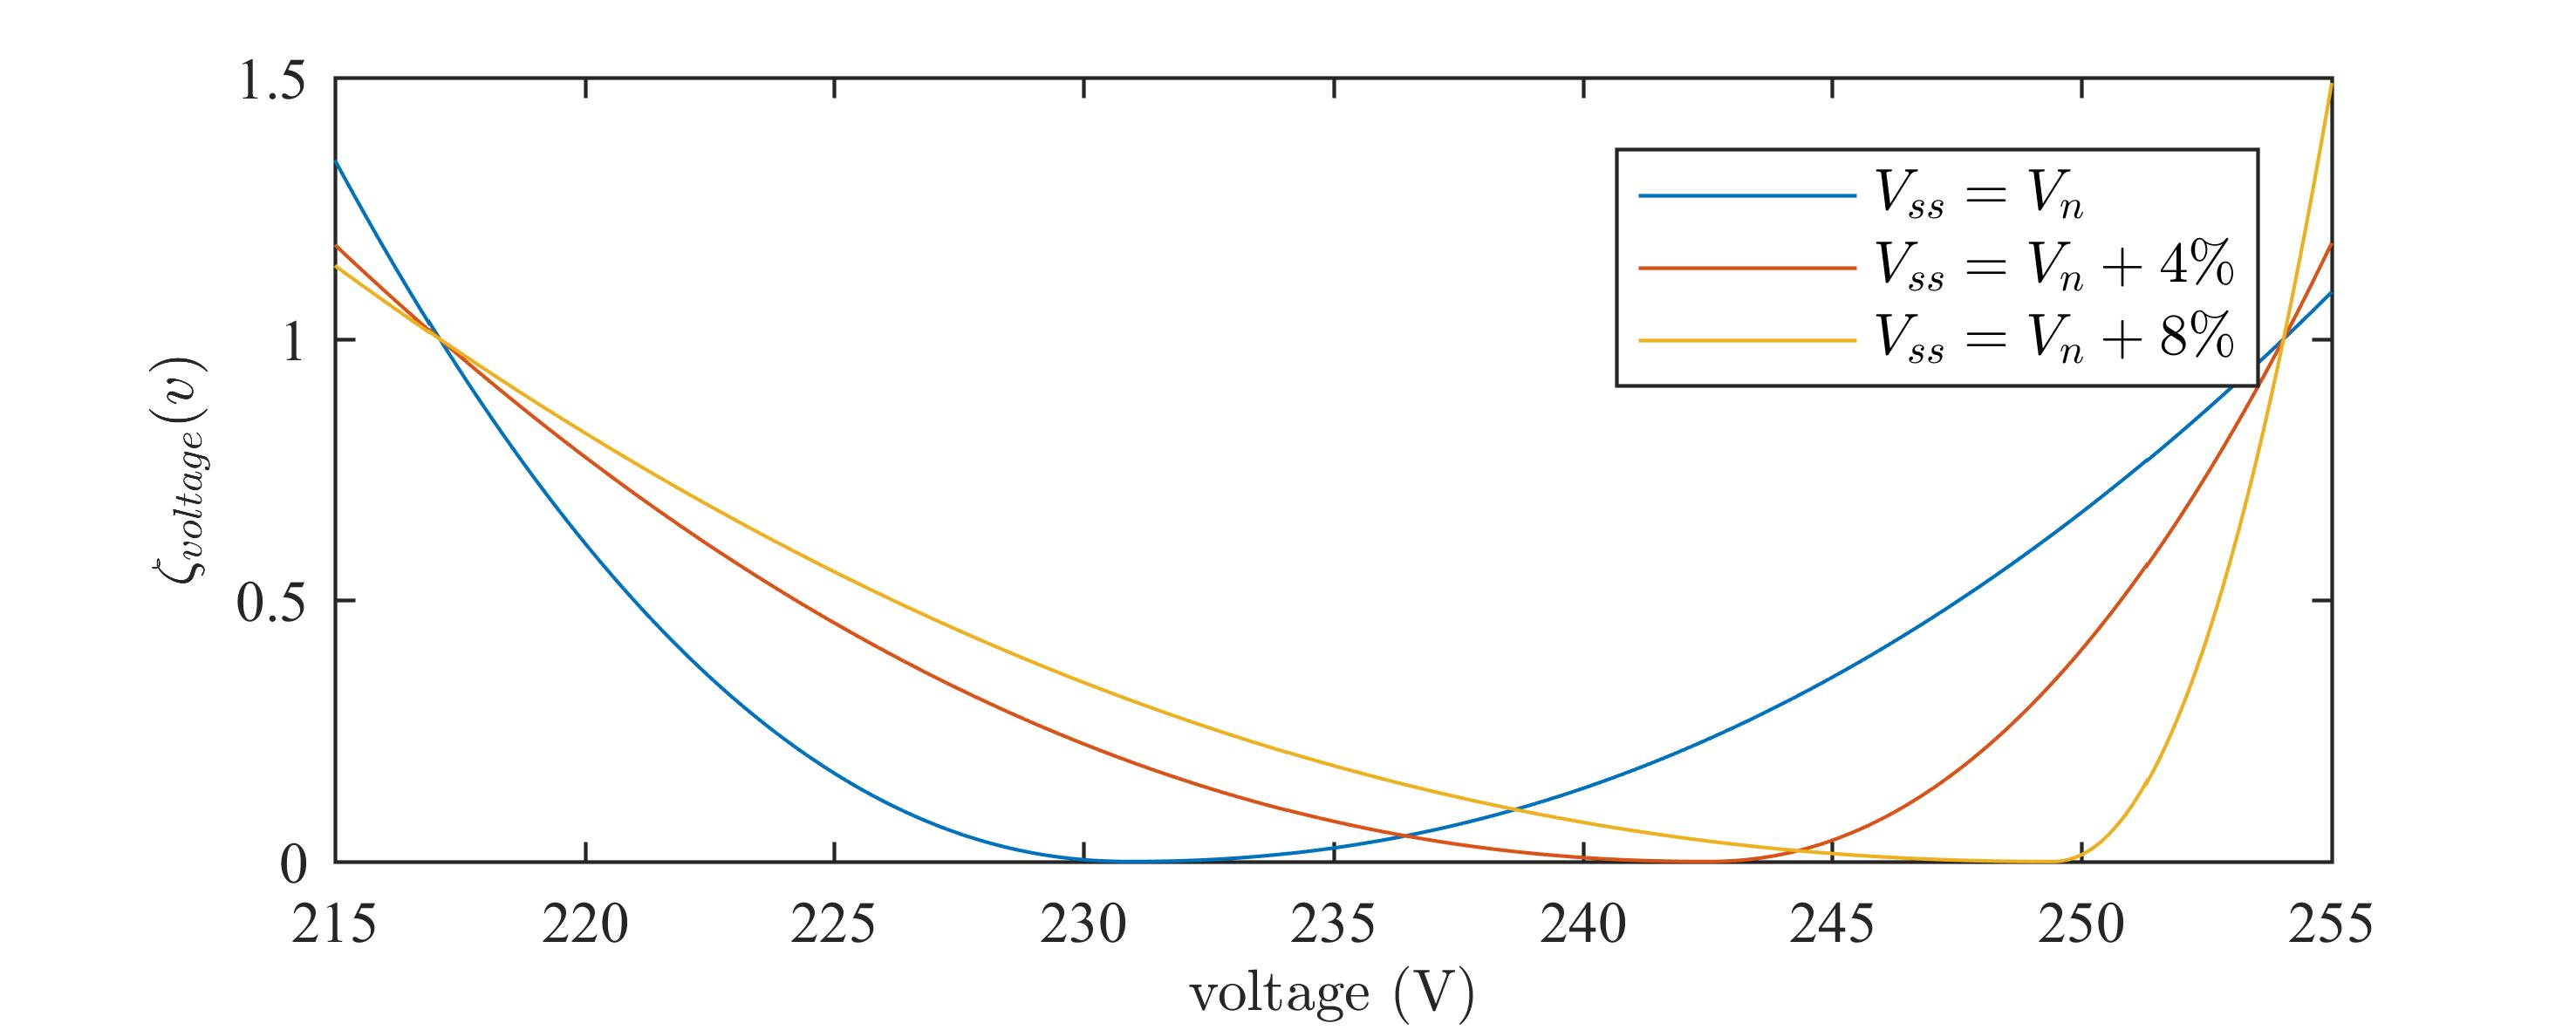
\includegraphics{_chapter1/fig/voltage-deviation}
	\caption{Cost function $\zeta_\text{voltage}(v_\phi)$ values for different substation voltages}	
	\label{ch1:fig:voltage-deviation}
\end{figure}

Here, it is shown that the cost at the high and low voltage thresholds equates to one, and zero at the set substation voltage.
When boosting this voltage, $V_{ss}$, only the zero point moved, whereas the high and low voltage crossings remain unchanged.
In Figure \ref{ch1:fig:voltage-deviation}, this behaviour is demonstrated by boosting $V_{ss}$ by +4\% and +8\%.

\subsection{Voltages at ESMU's PCC}
\label{ch1:subsec:voltages-at-esmu}

The ESMU is connected to all three phases of the feeder at some distance to the substation.
Where to connect the ESMU, in order to achieve an optimal network impact, is explained in Section \ref{ch1:sec:data-and-network-models}.
Ignoring the exact ESMU location, voltage along the line, i.e. from the substation to its PCC, will change and most likely drop.
The reason behind this effect is due to resistive losses in the lines, which are caused by the aggregative load currents.
For purely consumptive loads under heavy load conditions, this voltage may drop below the low-voltage threshold.
As mentioned in literature, this threshold is an operational constraint of LV networks and must not be violated to assure correct appliance operation.

In order to mitigate this voltage drop, power can be injected into the feeder at the ESMU's PCC.
Doing so boosts the voltage at that location since the portion of the load current, which would normally be supplied by the substation, is delivered by the ESMU.
The effect of this power injection is sketched below.

\begin{figure}\centering
	\subfloat[Voltage drop along feeder without ESMU intervention]{%
		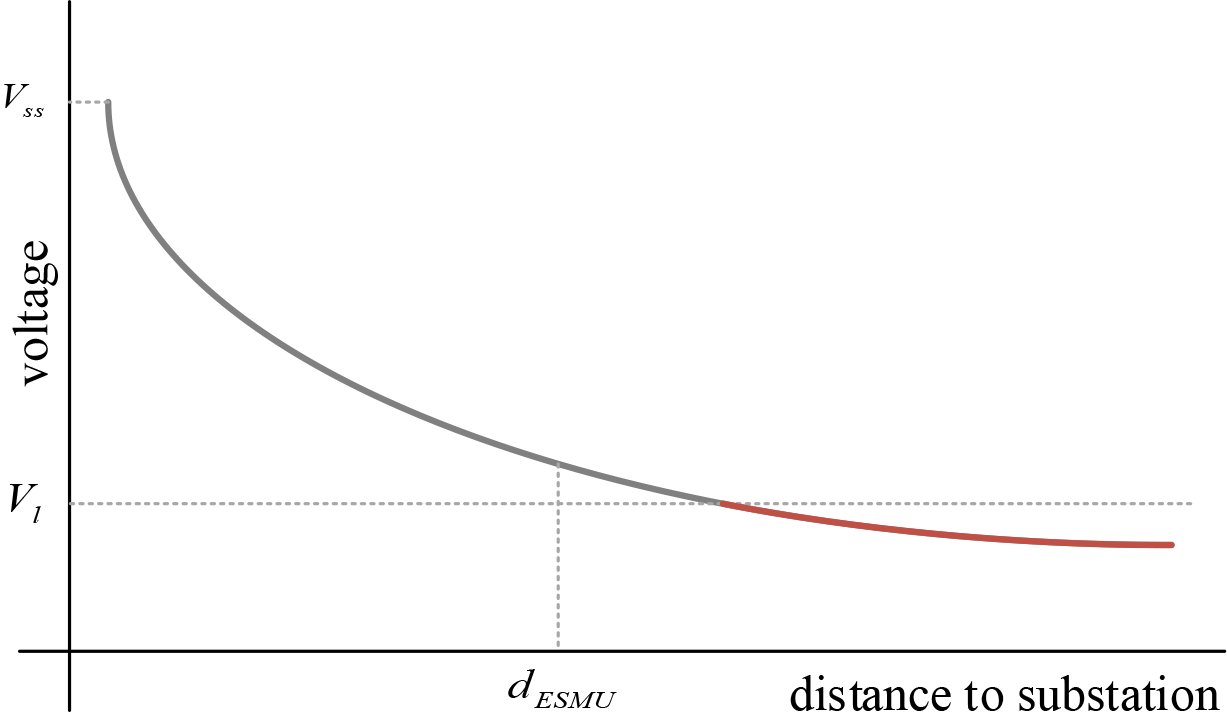
\includegraphics[width=0.45\textwidth]{_chapter1/fig/sketch-voltage-esmu-normal}%
		\label{ch1:subfig:sketch-voltage-esmu-normal}%
		}
	\hspace{5mm}
	\subfloat[Voltage drop along feeder with ESMU intervention]{%
		
\includegraphics[width=0.45\textwidth]{_chapter1/fig/sketch-voltage-esmu-boost}%
		\label{ch1:subfig:sketch-voltage-esmu-boost}%
		}
	\caption{Benefits of ESMU power injection on the voltage drop along the feeder}
	\label{ch1:fig:sketch-voltage-esmu}
\end{figure}

In Figure \ref{ch1:subfig:sketch-voltage-esmu-normal}, an expected voltage drop along the feeder is sketched, where the trailing feeder section's voltage dropped below $V_l$.
In contrast, Figure \ref{ch1:subfig:sketch-voltage-esmu-boost} shows how the ESMU intervention would alleviate some load and raise the trailing voltage levels to a level above $V_l$.

Since the P2N voltage at the ESMU's PCC can be measured quite easily, this realistic key network parameter is used in a cost function, too.
In fact, the ESMU's PCC voltage, $v_{ESMU,p}(t)$, is used in with Equation \ref{ch1:equ:voltage-deviation}; the same cost used for the substation transformer's secondary voltage.
Therefore, the resulting cost can be formulated as $\zeta_\text{voltage}(v_{ESMU,p}(t)) \forall t$.

\subsection{Voltages at customer laterals}
\label{ch1:subsec:voltages-at-customers}

Voltages at the customer are regulated in the UK, yet monitoring them in real-time is costly, and therefore they are not monitored.
Yet it is those voltages that are regulated and need to be kept within operational bands.
Ultimately, when it comes to voltage level correction, only substation voltage levels and customer voltage levels need to be controlled.
This fact is to assure proper transformer operation (e.g. to maximise its operation life) and to prevent penalisation due to customer voltage violation (i.e. fining according to ESQCR).
As shown in Section \ref{ch1:subsec:voltages-at-esmu}, ESMU can impact voltage levels for all customers, yet these voltage levels cannot be measured in reality.
In simulations however, extracting load voltages is easy, which is why they are treated as theoretical key network parameters.

To illustrate this load voltage drop, a sample OpenDSS simulation was run on the IEEE LV Test Case with all load powers set to an arbitrary value, i.e. 8kW.
When plotting the load bus voltage magnitudes against the distance between the load and its feeding substation the following plot is the result:

\begin{figure}\centering
	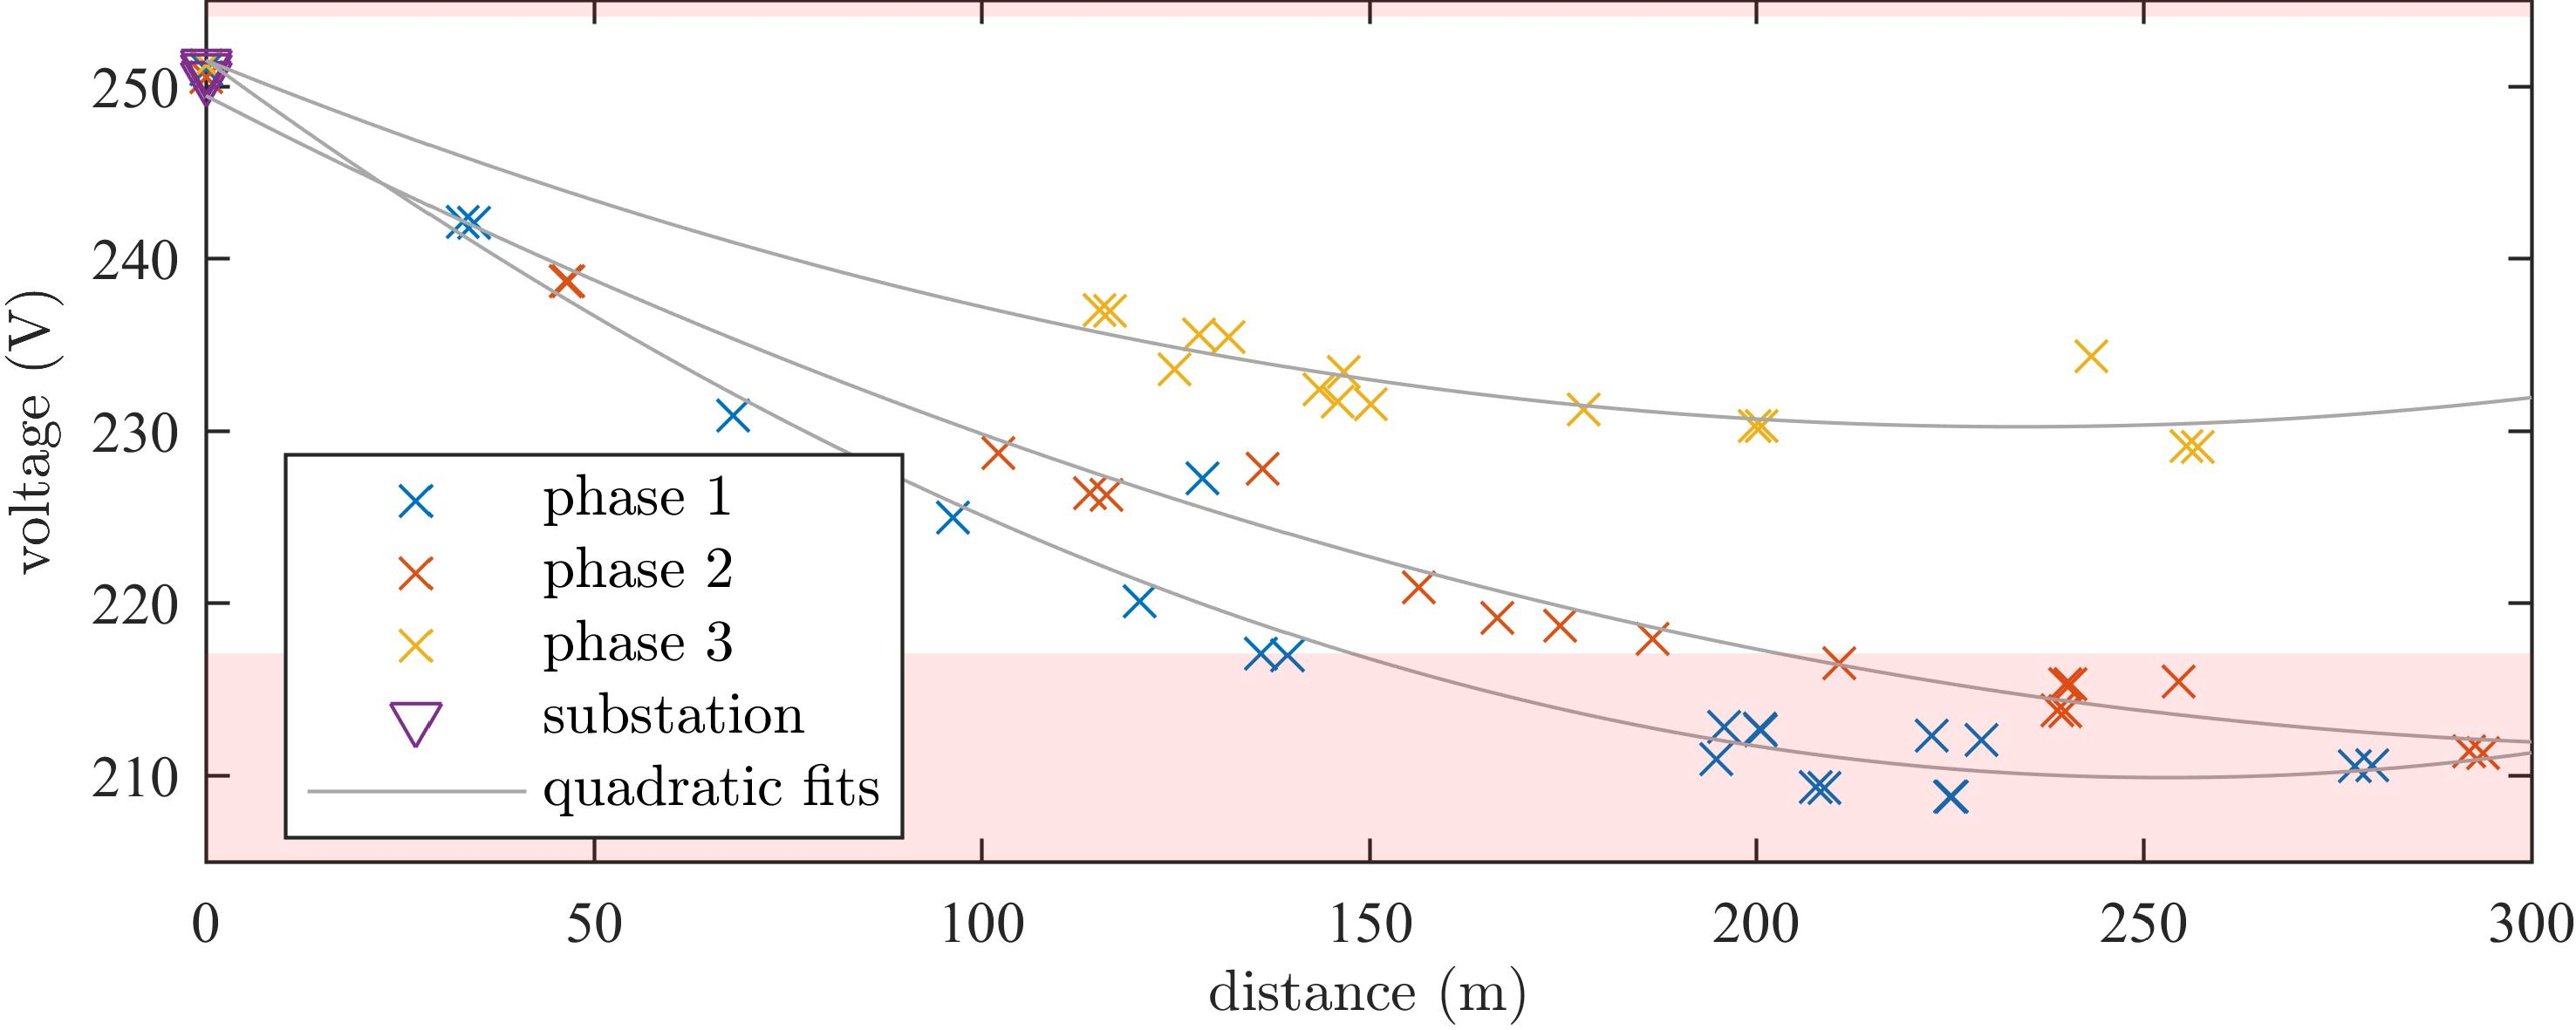
\includegraphics{_chapter1/fig/voltage-drop-for-loads-along-feeder}
	\caption{Voltage at the loads in the IEEE LV Test Case network for a total load of 440kVA against distance between the corresponding load and substation: for the quadratic fit $R^2=58.76\%$}
	\label{ch1:fig:voltage-drop-for-loads-along-feeder}
\end{figure}

In Figure \ref{ch1:fig:voltage-drop-for-loads-along-feeder}, it can be seen that phases are significantly unbalanced, and customers further than 200m from the substation would experience low-voltage events (for this particular scenario).
As already proposed in the previous section, ESMU aims to avoid these voltage violations, but the number of loads adds computational burden on the used solving algorithms.

To address this problem, the previously defined voltage cost function is expanded.
In fact, rather than including every single customer's voltage deviation cost, only the worst deviations are included.
By limiting this number, solvers need not consider such a large number of output parameters and only focus on the worst network parameter.
This focus is of particular need if the impact of the ESMU on some customers voltages is relatively low.
For this work, the customer (or load) voltage is defined as $\textbf{v}_{load}(t)$ (where $v_{load,i,p} \in \textbf{v}_{load}$) and used in the new cost function, $\zeta_\text{load voltage}(\textbf{v}_{load}(t)) \forall t$, as such:

\begin{equation}
\begin{split}
	\zeta_\text{load voltage}(\textbf{v}(t)) := \max_{i,\phi}{\zeta_\text{voltage}(v_{i,p}(t))} \\
	\text{ where } i \in \{1, \dots I\} \text{ and } \phi \in \{1, \dots, \Phi\} \text{ and } I \in \mathbb{Z}_{>0} \text{ and } \Phi \in \mathbb{Z}_{>0}
\end{split}
\label{ch1:equ:load-voltage-deviation}
\end{equation}

\subsection{Total power flow}
\label{ch1:subsec:total-power-flow}

As mentioned above, voltage deviation has an immediately perceptible effect on the network operation and violation of the predetermined voltage bands may even lead to financial penalisation.
Since all possible means of limiting voltage divergence have been addressed (in the scope of this work) further network parameters are put into focus next.
A not yet considered network parameter, that also impacts the effective network operation, is power flow into the network, or more specifically; the power flow in each of the three phases of the distribution feeder.
Customers in urban UK distribution networks have a single phase connection to the three-phase feeder line (this is done by connecting their supply cables or ``laterals'' between a phase and the neutral conductor).
In the UK, the procedure for connecting customers is done in a somewhat arbitrary manner in order to distribute load as evenly as possible across all three phases.
In theory, this approach assures a balanced network load, yet in reality this is not the case.
Even if the number of customers per phase was the same for each individual phase, the probability that all customers' load profiles are identical is very low.
Therefore, the likeliness of LV distribution feeders to be unbalanced is very high.
Unbalance can be calculated from substation the phase powers, as they are monitored at the substation.

Unlike the aforementioned voltage deviations, unbalance does not directly impact customer.
Nonetheless, unbalance is a network disturbance that has significant impact on the efficiency and long term reliability of three-phase components (e.g. rotating machines and transformers).
Phase unbalance itself is unavoidable and has no direct negative impact on network operation, yet reducing the magnitude of the unbalance plays a more important role in network optimisation.
Therefore a standardised measure of unbalance was developed and is used in the presented work, too \cite{ANSI-MB-1-2011}.
An Unbalance Factor, $\text{UF}(\textbf{x})$, is therefore defined as:

\begin{equation}
	\text{UF}(\textbf{x}) := \frac{\max_n |\bar{\textbf{x}} - x_n|}{\bar{\textbf{x}}}
	\label{ch1:equ:unbalance-equation}
\end{equation}

Here, $\textbf{x}$ is a three phase vector, where $x_n \in \textbf{x} \text{ for } n=[1, 2, 3]$.
$x_n$ may be a voltage, current or power measurement per phase, but for context of this work $x_n$ was chosen to be the power flow into the network.
For clarity, the notation $\bar{\textbf{s}}$ is used to define the mean of all three phase values.
The mean's definition is give below:

\begin{equation}
	\bar{\textbf{x}} := \frac{1}{3}\sum_n^3{x_i}
\end{equation}

Substation power readings, $\textbf{s}_{ss}(t)$, are used to calculate the phase unbalance to serve as another key network parameter.
Therefore, the unbalance factor in Equation \ref{ch1:equ:unbalance-equation} was included in another cost function.
Since the minimum value of $\text{UF}(\textbf{s}_{ss})$ is 1, an adjustment was required so that a perfectly balance network would result in an $\text{UF}(\textbf{s}_{ss})$ of zero.
The cost function is defined as $\zeta_\text{unbalance}(\textbf{s}_{ss}) \forall t$,  where $s_{ss,p} \in \textbf{s}_{ss}$:

\begin{equation}
	\begin{split}
		\zeta_\text{unbalance}(\textbf{s}(t)):=&\text{UF}(\textbf{s}(t)) - 1 \forall t\\
		=&\frac{\max_p\left|\overline{\textbf{s}(t)} - s_{p}(t)\right|}{\overline{\textbf{s}(t)}} \forall t\\
		=&\frac{\max_p\left|\left(\frac{1}{P}\sum_p^P{s_{p}(t)}\right) - s_{p}(t)\right|}{\frac{1}{P}\sum_p^P{s_{p}(t)}} \forall t\\
		&\text{where } p \in [1, 2, \dots P]
	\end{split}
	\label{ch1:equ:unbalance-cost}
\end{equation}


An illustration how this cost function is provided in the figure below.

\begin{figure}\centering
	
\includegraphics[width=5cm]{foo}
	\caption{Sample network imbalance for different phase loadings as defined in ANSI/NEMA MG 1-2011}
	\label{ch1:fig:power-unbalance}
\end{figure}

Here, it can be seen how $\zeta_\text{unbalance}$ varies with an increasing separation of the three phases' power values.

\subsection{Line utilisation}
\label{ch1:subsec:line-utilisation}

Inline with power, total power demand puts strain on the feeding cable, since resistive losses cause cable heating.
Hence, cables have been assigned a certain thermal rating which must not be exceeded to prevent cable damage and network failures.
The dissipated power, which leads to the cable's heating and failure, is a function in respect of the entire cable's properties.
Yet means of measuring those cable properties instantaneously are still being research and not industry ready.
Therefore, the most common approach to identify the loading of a cable is by comparing its present current flow against the its nominal amperage rating.

For the context of this work, this nominal rating, $i_{nom,l}$, is a fixed value for each cable type and is the total current that may flow through a cable before its maximum thermal rating is exceeded.
A subsequent cost function therefore needs to find the total current first, before comparing it to the line's rating.
This so called utilisation cost function $\zeta_\text{utilisation}(\textbf{i}_{line}(t)) \forall t$ is a function of the three phase line current $\textbf{i}_{line}$ (where $i_{line,l,p} \in \textbf{i}_{line}$) and is defined as:

\begin{equation}
	\zeta_\text{utilisation}(\textbf{i}_{line}) := \max_l{\frac{\sum_p^3i_{line,l,p}}{i_{nom,l}}}
	\label{ch1:equ:cable-utilisation}
\end{equation}

\subsection{Distribution losses}
\label{ch1:subsec:losses}





